\documentclass[xetex,mathserif,serif]{beamer}
\usepackage{polyglossia}
\setdefaultlanguage[babelshorthands=true]{russian}
\usepackage{minted}
\usepackage{tabu}
\usepackage[11pt]{moresize}

\usepackage{textpos}
\setlength{\TPHorizModule}{1cm}
\setlength{\TPVertModule}{1cm}

\useoutertheme{infolines}

\usepackage{fontspec}
\setmainfont{FreeSans}
\newfontfamily{\russianfonttt}{FreeSans}

\tabulinesep=0.7mm

\newcommand{\attribution}[1] {
	\begin{flushright}\begin{scriptsize}\textcolor{gray}{\textcopyright\; #1}\end{scriptsize}\end{flushright}
}

\title{Проектирование распределённых приложений}
\subtitle{Часть вторая: высокоуровневые вещи}
\author[Юрий Литвинов]{Юрий Литвинов \newline \textcolor{gray}{\small\texttt{yurii.litvinov@gmail.com}}}

\date{14.12.2017}

\begin{document}
	
	\frame{\titlepage}

	\section{Docker}

	\begin{frame}
		\frametitle{Docker}
		\begin{itemize}
			\item Средство для ``упаковки'' приложений в изолированные контейнеры
			\item Что-то вроде легковесной виртуальной машины
		\end{itemize}
		\begin{center}
			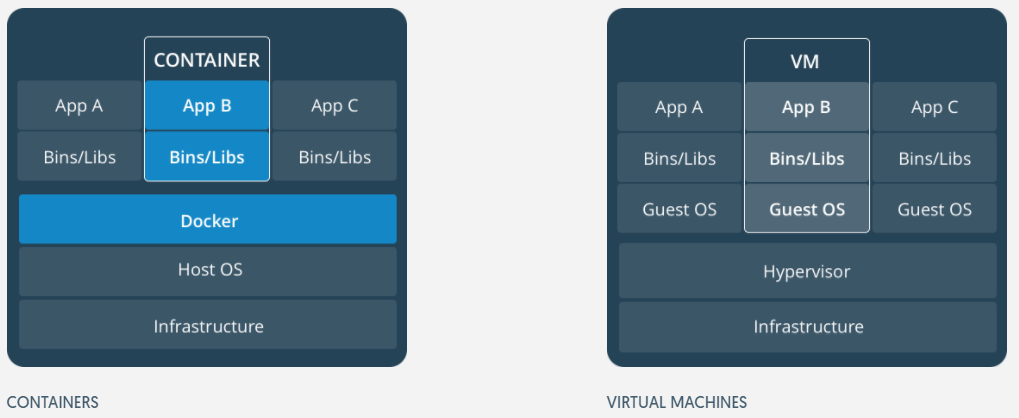
\includegraphics[width=0.7\textwidth]{docker.png}
			\attribution{\url{https://www.docker.com}}
		\end{center}
	\end{frame}
	
	\begin{frame}[fragile]
		\frametitle{Dockerfile}
		\begin{scriptsize}
			\begin{minted}{sh}
# Use an official Python runtime as a parent image
FROM python:2.7-slim

# Set the working directory to /app
WORKDIR /app

# Copy the current directory contents into the container at /app
ADD . /app

# Install any needed packages specified in requirements.txt
RUN pip install --trusted-host pypi.python.org -r requirements.txt

# Make port 80 available to the world outside this container
EXPOSE 80

# Define environment variable
ENV NAME World

# Run app.py when the container launches
CMD ["python", "app.py"]
			\end{minted}
		\end{scriptsize}
	\end{frame}

	\begin{frame}[fragile]
		\frametitle{Балансировка нагрузки}
		\framesubtitle{docker-compose.yml}
		\begin{scriptsize}
			\begin{minted}{yaml}
version: "3"
services:
    web:
        # replace username/repo:tag with your name and image details
        image: username/repo:tag
        deploy:
            replicas: 5
            resources:
                limits:
                    cpus: "0.1"
                    memory: 50M
            restart_policy:
                condition: on-failure
        ports:
            - "80:80"
        networks:
            - webnet
networks:
    webnet:
			\end{minted}
		\end{scriptsize}
	\end{frame}

	\begin{frame}
		\frametitle{Swarm-ы}
		\begin{itemize}
			\item Машина, на которой запускается контейнер, становися главной
			\item Другие машины могут присоединяться к swarm-у и получать копию контейнера
			\item Docker балансирует нагрузку по машинам
		\end{itemize}
		\begin{center}
			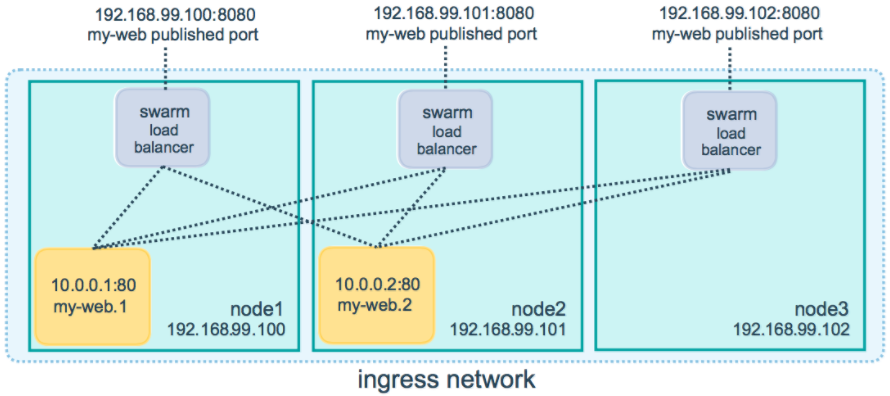
\includegraphics[width=0.7\textwidth]{swarmLoadBalancing.png}
			\attribution{\url{https://www.docker.com}}
		\end{center}
	\end{frame}

	\section{SOAP}

	\begin{frame}
		\frametitle{SOAP-ориентированные сервисы}
		\begin{columns}
			\begin{column}{0.6\textwidth}
				\begin{itemize}
					\item Simple Object Access Protocol
					\item Web Services Description Language
					\item Universal Discovery, Description and Integration
				\end{itemize}
			\end{column}
			\begin{column}{0.4\textwidth}
				\begin{center}
					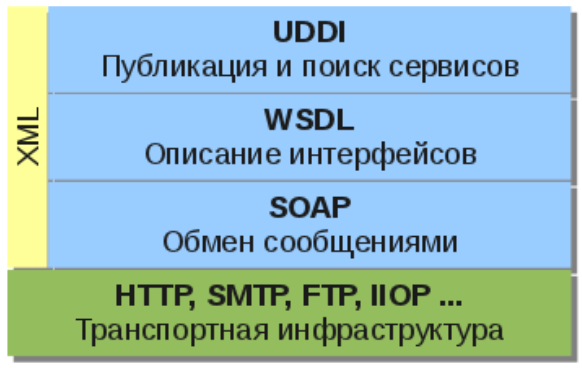
\includegraphics[width=\textwidth]{soap.png}
				\end{center}
			\end{column}
		\end{columns}
	\end{frame}

	\begin{frame}[fragile]
		\frametitle{SOAP-сообщение}
		\begin{small}
			\begin{minted}{xml}
<env:Envelope xmlns:env="http://www.w3.org/2003/05/soap-envelope">
    <env:Header>
        <n:alertcontrol xmlns:n="http://example.org/alertcontrol">
            <n:priority>1</n:priority>
            <n:expires>2001-06-22T14:00:00-05:00</n:expires>
        </n:alertcontrol>
    </env:Header>
    <env:Body>
        <m:alert xmlns:m="http://example.org/alert">
            <m:msg>Get up at 6:30 AM</m:msg>
        </m:alert>
    </env:Body>
</env:Envelope>
			\end{minted}
		\end{small}
	\end{frame}

	\begin{frame}[fragile]
		\frametitle{WSDL-описание}
		\begin{small}
			\begin{minted}{xml}
<message name="getTermRequest">
    <part name="term" type="xs:string"/>
</message>

<message name="getTermResponse">
    <part name="value" type="xs:string"/>
</message>

<portType name="glossaryTerms">
    <operation name="getTerm">
        <input message="getTermRequest"/>
        <output message="getTermResponse"/>
    </operation>
</portType>
			\end{minted}
		\end{small}
	\end{frame}

	\begin{frame}
		\frametitle{Достоинства SOAP-based сервисов}
		\begin{itemize}
			\item Автоматический режим описания сервисов
			\item Автоматическая поддержка описаний SOAP-клиентом
			\item Автоматическая валидация сообщений
			\begin{itemize}
				\item Валидность xml
				\item Проверка по схеме
				\item Проверка SOAP-сервером
			\end{itemize}
			\item Работа через HTTP
			\begin{itemize}
				\item Хоть через обычный GET
			\end{itemize}
		\end{itemize}
	\end{frame}

	\begin{frame}
		\frametitle{Недостатки SOAP-based сервисов}
		\begin{itemize}
			\item Огромный размер сообщений
			\item Сложность описаний на клиенте и сервере
			\item Один запрос --- один ответ
			\begin{itemize}
				\item Поддержка транзакций на уровне бизнес-логики
			\end{itemize}
			\item Сложности миграции при изменении описания
		\end{itemize}
	\end{frame}

	\section{WCF}

	\begin{frame}
		\frametitle{Пример: WCF}
		\begin{itemize}
			\item Платформа для создания веб-сервисов
			\item Часть .NET Framework, начиная с 3.0
			\item Умеет WSDL, SOAP и т.д., очень конфигурируема
			\item Автоматическая генерация заглушек на стороне клиента
			\item ABCs of WCF:
			\begin{itemize}
				\item Address
				\item Binding
				\item Contract
			\end{itemize}
		\end{itemize}
		\begin{center}
			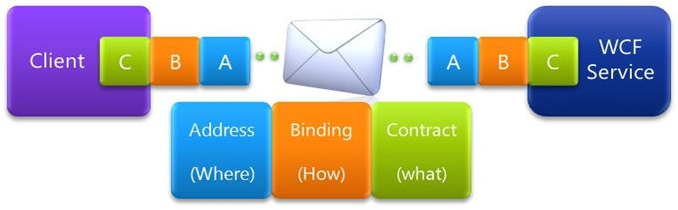
\includegraphics[width=0.6\textwidth]{wcf.png}
			\attribution{\url{http://www.c-sharpcorner.com}}
		\end{center}
	\end{frame}

	\begin{frame}[fragile]
		\frametitle{Пример, описание контракта}
		\begin{small}
			\begin{minted}{csharp}
[ServiceContract(Namespace = "http://Microsoft.ServiceModel.Samples")]  
public interface ICalculator  
{
    [OperationContract]
    double Add(double n1, double n2);

    [OperationContract]
    double Subtract(double n1, double n2);

    [OperationContract]
    double Multiply(double n1, double n2);

    [OperationContract]
    double Divide(double n1, double n2);
}
			\end{minted}
		\end{small}
	\end{frame}

	\begin{frame}[fragile]
		\frametitle{Пример, реализация контракта}
		\begin{small}
			\begin{minted}{csharp}
public class CalculatorService : ICalculator  
{
    public double Add(double n1, double n2)
        => n1 + n2;  

    public double Subtract(double n1, double n2)
        => n1 - n2

    public double Multiply(double n1, double n2)  
        => n1 * n2;

    public double Divide(double n1, double n2)  
        => n1 / n2;
}
			\end{minted}
		\end{small}
	\end{frame}

	\begin{frame}[fragile]
		\frametitle{Пример, self-hosted service}
		\begin{scriptsize}
			\begin{minted}{csharp}
static void Main(string[] args) 
{
    Uri baseAddress = new Uri("http://localhost:8000/ServiceModelSamples/Service");
    ServiceHost selfHost = new ServiceHost(typeof(CalculatorService), baseAddress);

    try {
        selfHost.AddServiceEndpoint(typeof(ICalculator), new WSHttpBinding(), "CalculatorService");

        ServiceMetadataBehavior smb = new ServiceMetadataBehavior();
        smb.HttpGetEnabled = true;
        selfHost.Description.Behaviors.Add(smb);

        selfHost.Open();
        Console.WriteLine("The service is ready. Press <ENTER> to terminate service.");
        Console.ReadLine();

        selfHost.Close();  
    } catch (CommunicationException ce) {
        Console.WriteLine($"An exception occurred: {ce.Message}");
        selfHost.Abort();
    }
}
			\end{minted}
		\end{scriptsize}
	\end{frame}

	\begin{frame}[fragile]
		\frametitle{Пример, клиент}
		\begin{itemize}
			\item Генерация заглушки: 
				\begin{scriptsize}
					\begin{minted}{text}
svcutil.exe /language:cs /out:generatedProxy.cs /config:app.config^
    http://localhost:8000/ServiceModelSamples/service
					\end{minted}
				\end{scriptsize}
			\item Клиент:
				\begin{footnotesize}
					\begin{minted}{csharp}
static void Main(string[] args)
{
    CalculatorClient client = new CalculatorClient();

    double value1 = 100.00D;
    double value2 = 15.99D;
    double result = client.Add(value1, value2);
    Console.WriteLine($"Add({value1},{value2}) = {result}");

    client.Close();
}
					\end{minted}
				\end{footnotesize}
		\end{itemize}
	\end{frame}

	\begin{frame}[fragile]
		\frametitle{Пример, конфигурация клиента}
		\begin{ssmall}
			\begin{minted}{xml}
<?xml version="1.0" encoding="utf-8" ?>  
<configuration>  
    <startup>   
      <!-- specifies the version of WCF to use-->  
        <supportedRuntime version="v4.0" sku=".NETFramework,Version=v4.5,Profile=Client" />  
    </startup>  
    <system.serviceModel>  
        <bindings>  
            <!-- Uses wsHttpBinding-->  
            <wsHttpBinding>  
                <binding name="WSHttpBinding_ICalculator" />  
            </wsHttpBinding>  
        </bindings>  
        <client>  
            <!-- specifies the endpoint to use when calling the service -->  
            <endpoint address="http://localhost:8000/ServiceModelSamples/Service/CalculatorService"  
                binding="wsHttpBinding" bindingConfiguration="WSHttpBinding_ICalculator"  
                contract="ServiceReference1.ICalculator" name="WSHttpBinding_ICalculator">  
                <identity>  
                    <userPrincipalName value="migree@redmond.corp.microsoft.com" />  
                </identity>  
            </endpoint>  
        </client>  
    </system.serviceModel>  
</configuration>
			\end{minted}
		\end{ssmall}
	\end{frame}

	\section{Очереди сообщений}

	\begin{frame}
		\frametitle{Очереди сообщений}
		\begin{itemize}
			\item Используются для гарантированной доставки сообщений
			\begin{itemize}
				\item Даже если отправитель и получатель доступны в разное время
				\item Локальное хранилище сообщений на каждом устройстве
			\end{itemize}
			\item Реализуют модель ``издатель-подписчик'', но могут работать и в режиме ``точка-точка''
			\item Как правило, имеют развитые возможности маршрутизации, фильтрации и преобразования сообщений
			\begin{itemize}
				\item Разветвители, агрегаторы, преобразователи порядка
			\end{itemize}
		\end{itemize}
	\end{frame}

	\section{RabbitMQ}

	\begin{frame}
		\frametitle{RabbitMQ}
		\begin{itemize}
			\item Сервер и клиенты системы надёжной передачи сообщений
			\begin{itemize}
				\item Сообщение посылается на сервер и хранится там, пока его не заберут
				\item Продвинутые возможности по маршрутизации сообщений
			\end{itemize}
			\item Реализует протокол AMQP (Advanced Message Queuing Protocol), но может использовать и другие протоколы
			\item Сервер написан на Erlang, клиентские библиотеки доступны для практически чего угодно
		\end{itemize}
		\begin{textblock}{3}(8,0)
			
\includegraphics[width=\textwidth]{rabbitmqLogo.png}
		\end{textblock}
	\end{frame}

	\begin{frame}[fragile]
		\frametitle{Пример, отправитель}
		\begin{ssmall}
			\begin{minted}{csharp}
using System;
using RabbitMQ.Client;
using System.Text;

class Send
{
    public static void Main()
    {
        var factory = new ConnectionFactory() { HostName = "localhost" };
        using (var connection = factory.CreateConnection())
        {
            using (var channel = connection.CreateModel())
            {
                channel.QueueDeclare(queue: "hello", durable: false, exclusive: false,
                                     autoDelete: false, arguments: null);

                string message = "Hello World!";
                var body = Encoding.UTF8.GetBytes(message);

                channel.BasicPublish(exchange: "", routingKey: "hello",
                                     basicProperties: null, body: body);
            }
        }
    }
}
			\end{minted}
		\end{ssmall}
	\end{frame}

	\begin{frame}[fragile]
		\frametitle{Пример, получатель}
		\begin{ssmall}
			\begin{minted}{csharp}
using RabbitMQ.Client;
using RabbitMQ.Client.Events;
using System;
using System.Text;

class Receive
{
    public static void Main()
    {
        var factory = new ConnectionFactory() { HostName = "localhost" };
        using (var connection = factory.CreateConnection())
        using (var channel = connection.CreateModel())
        {
            channel.QueueDeclare(queue: "hello", durable: false, exclusive: false, autoDelete: false, arguments: null);

            var consumer = new EventingBasicConsumer(channel);
            consumer.Received += (model, ea) =>
            {
                var body = ea.Body;
                var message = Encoding.UTF8.GetString(body);
                Console.WriteLine(" [x] Received {0}", message);
            };
            channel.BasicConsume(queue: "hello", autoAck: true, consumer: consumer);
        }
    }
}
			\end{minted}
		\end{ssmall}
	\end{frame}

	\section{ESB}

	\begin{frame}
		\frametitle{Enterprise Service Bus}
		\begin{center}
			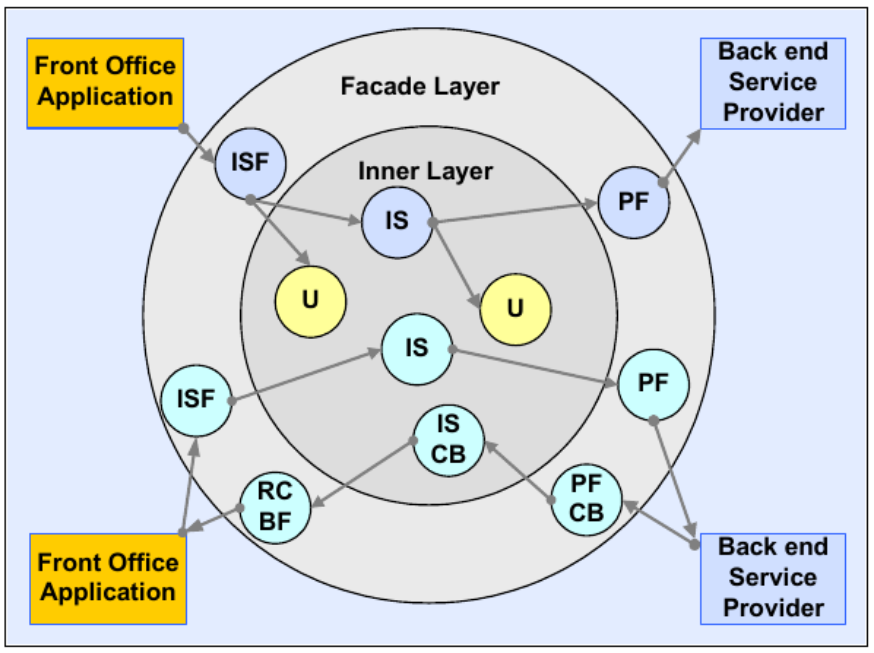
\includegraphics[width=0.7\textwidth]{esb.png}
		\end{center}
	\end{frame}

	\section{REST}

	\begin{frame}
		\frametitle{Representational State Transfer (REST)}
		\begin{itemize}
			\item Модель клиент-сервер
			\item Отсутствие состояния
			\item Кэширование
			\item Единообразие интерфейса
			\item Слои
		\end{itemize}
	\end{frame}

	\begin{frame}
		\frametitle{Интерфейс сервиса}
		\begin{itemize}
			\item Коллекции
			\begin{itemize}
				\item \url{http://api.example.com/resources/}
			\end{itemize}
			\item Элементы
			\begin{itemize}
				\item \url{http://api.example.com/resources/item/17}
			\end{itemize}
			\item HTTP-методы
			\begin{itemize}
				\item GET
				\item PUT
				\item POST
				\item DELETE
			\end{itemize}
			\item Передача параметров прямо в URL
			\begin{itemize}
				\item \url{http://api.example.com/resources?user=me&access_token=ASFQF}
			\end{itemize}
		\end{itemize}
	\end{frame}

	\begin{frame}
		\frametitle{Пример, Google Drive REST API}
		\begin{itemize}
			\item GET https://www.googleapis.com/drive/v2/files --- список всех файлов
			\item GET https://www.googleapis.com/drive/v2/files/fileId --- метаданные файла по его Id
			\item POST https://www.googleapis.com/upload/drive/v2/files — загрузить новый файл
			\item PUT https://www.googleapis.com/upload/drive/v2/files/fileId --- обновить файл
			\item DELETE https://www.googleapis.com/drive/v2/files/fileId --- удалить файл
		\end{itemize}
	\end{frame}

	\begin{frame}
		\begin{center}
			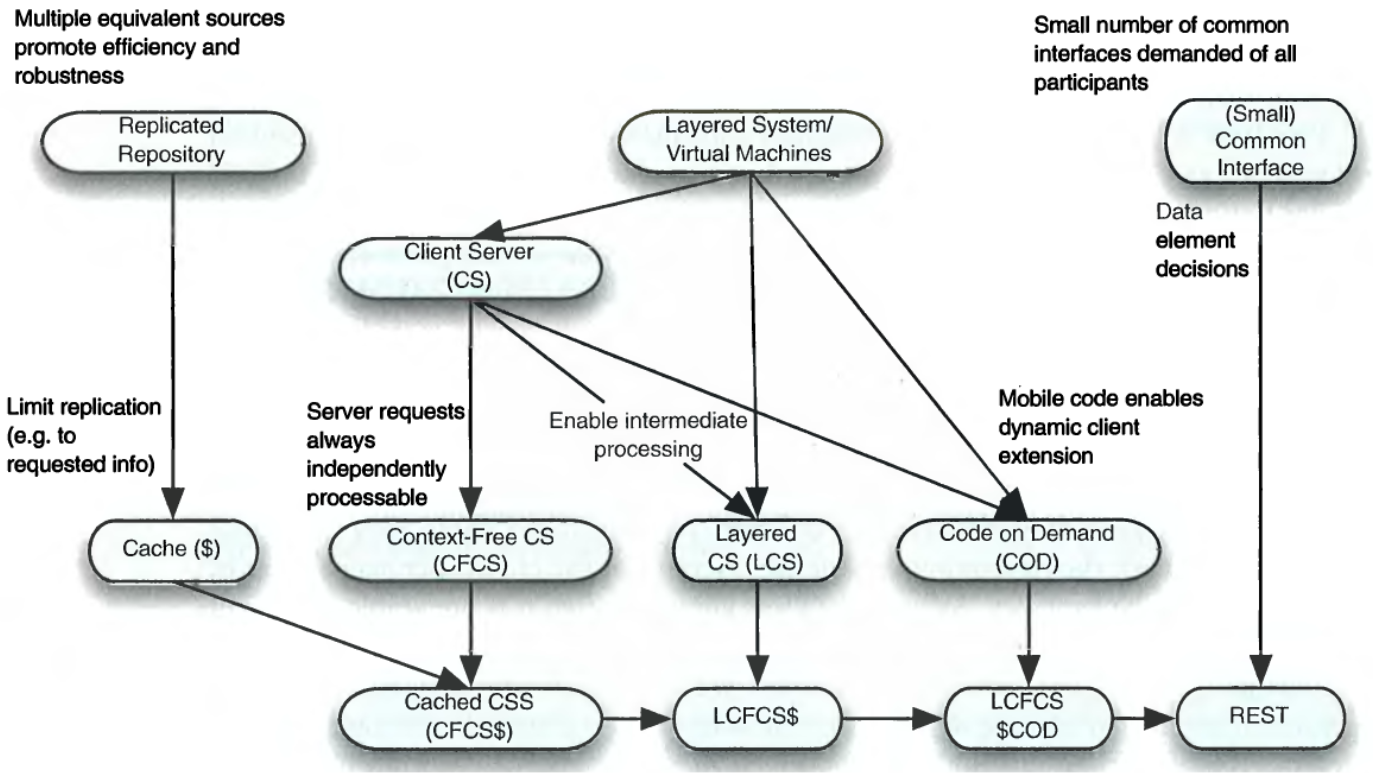
\includegraphics[width=\textwidth]{rest.png}
		\end{center}
	\end{frame}

	\begin{frame}
		\frametitle{Достоинства}
		\begin{itemize}
			\item Надёжность
			\item Производительность
			\item Масштабируемость
			\item Прозрачность системы взаимодействия
			\item Простота интерфейсов
			\item Портативность компонентов
			\item Лёгкость внесения изменений
		\end{itemize}
	\end{frame}

	\section{Микросервисы}

	\begin{frame}
		\frametitle{Микросервисы}
		\begin{itemize}
			\item Набор небольших сервисов
			\begin{itemize}
				\item Разные языки и технологии
			\end{itemize}
			\item Каждый в собственном процессе
			\begin{itemize}
				\item Независимое развёртывание
				\item Децентрализованное управление
			\end{itemize}
			\item Легковесные коммуникации
		\end{itemize}
	\end{frame}

	\begin{frame}
		\frametitle{Монолитные приложения}
		\begin{itemize}
			\item Большой и сложный MVC
			\item Единый процесс разработки и стек технологий
			\item Сложная архитектура
			\item Сложно масштабировать
			\item Сложно вносить изменения
		\end{itemize}
	\end{frame}

	\begin{frame}
		\frametitle{Разбиение на сервисы}
		\begin{center}
			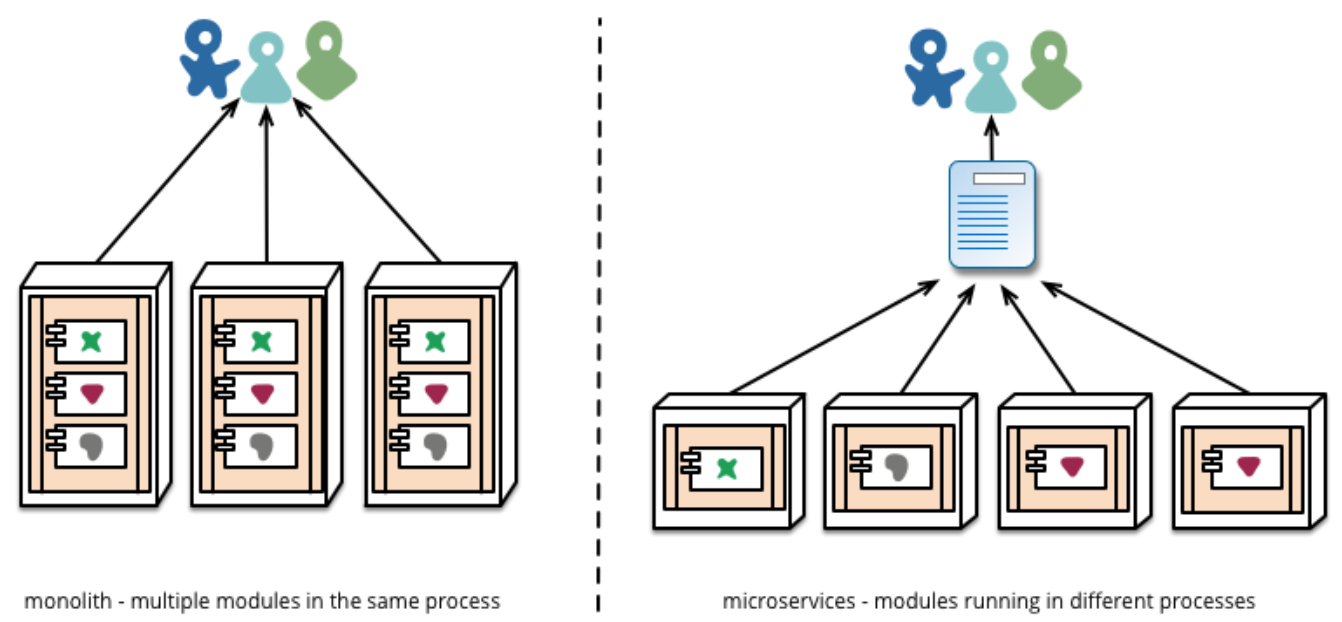
\includegraphics[width=\textwidth]{microservices.png}
		\end{center}
	\end{frame}

	\begin{frame}
		\frametitle{Основные особенности}
		\begin{itemize}
			\item Микросервисы и SOA
			\item Smart endpoints and dumb pipes
			\item Проектирование под отказ
			\item Асинхронные вызовы
			\item Децентрализованное управление данными
			\item Автоматизация инфраструктуры
			\item Эволюционный дизайн
		\end{itemize}
	\end{frame}

	\begin{frame}
		\frametitle{Основные проблемы}
		\begin{itemize}
			\item Сложности выделения границ сервисов
			\item Перенос логики на связи между сервисами
			\begin{itemize}
				\item Большой обмен данными
				\item Нетривиальные зависимости
			\end{itemize}
			\item Нетривиальная инфраструктура
			\item Нетривиальная переиспользуемость кода
		\end{itemize}
	\end{frame}

	\section{Peer-to-peer}

	\begin{frame}
		\frametitle{Архитектура Peer-to-Peer}
		\begin{itemize}
			\item Децентрализованный и самоорганизующийся сервис
			\item Динамическая балансировка нагрузки
			\begin{itemize}
				\item Вычислительные ресурсы
				\item Хранилища данных
			\end{itemize}
			\item Динамическое изменение состава участников
		\end{itemize}
	\end{frame}

	\begin{frame}
		\frametitle{Napster: hybrid client-server/P2P}
		\begin{center}
			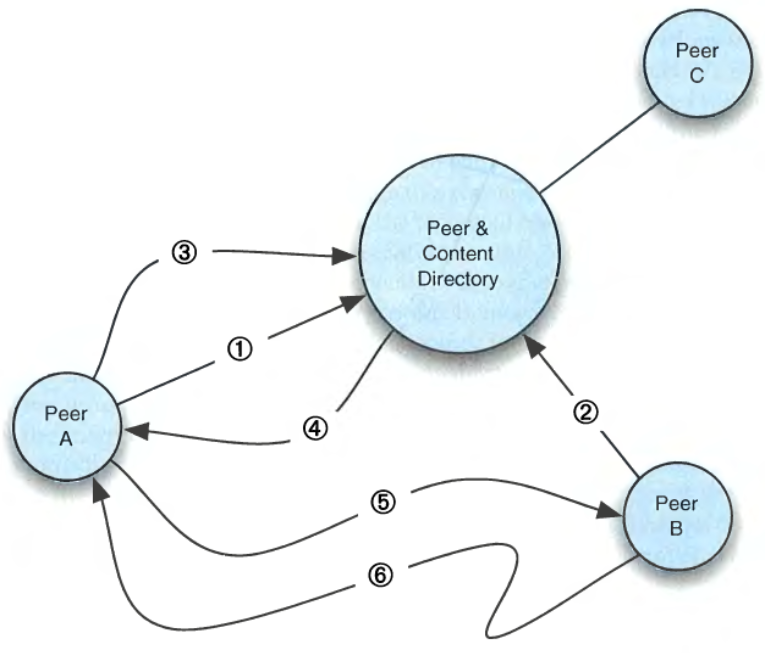
\includegraphics[width=0.6\textwidth]{napster.png}
		\end{center}
	\end{frame}

	\begin{frame}
		\frametitle{Skype: Overlayed P2P}
		\begin{center}
			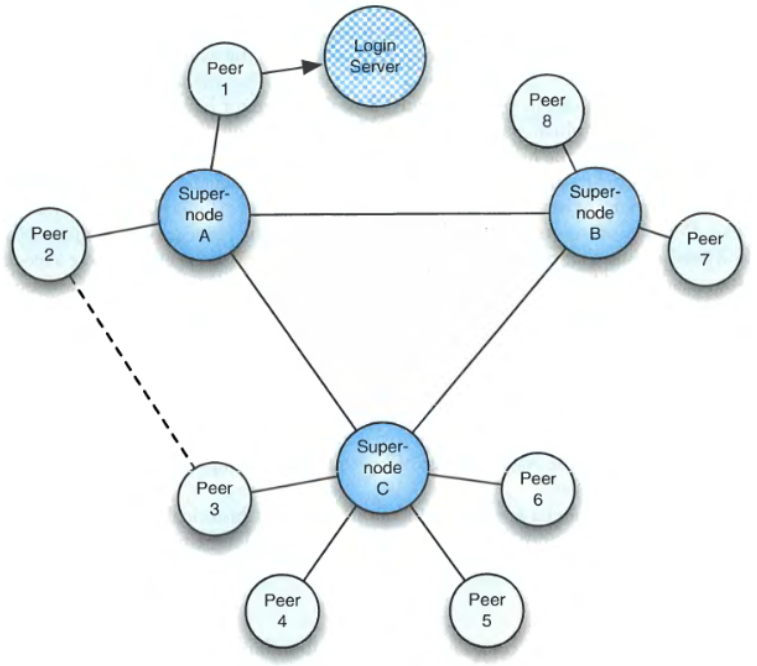
\includegraphics[width=0.6\textwidth]{skype.png}
		\end{center}
	\end{frame}

	\begin{frame}
		\frametitle{BitTorrent : Resource Trading P2P}
		\begin{itemize}
			\item Обмен сегментами
			\item Поиск не входит в протокол
			\item Трекеры
			\item Метаданные
			\item Управление приоритетами
			\item Бестрекерная реализация
		\end{itemize}
	\end{frame}

\end{document}
